
\chapter{Significance thresholds for exhaustive two dimensional testing}
\label{Results3}
\lhead{Chapter 4. \emph{Significance thresholds for exhaustive two dimensional testing}}

\section{Abstract}
\setstretch{1}
Genome wide association studies impose a heavy multiple testing penalty which is detrimental to their power, so the question of significance thresholds is important. In one dimensional scans this has been explored deeply, and it can be demonstrated that because of correlation between the SNPs being tested, the effective number of tests is much lower than the actual number performed. But the degree to which this is the case in two dimensional searches for epistasis has been difficult to determine because of computational obstacles. With the emergence of GPGPU clusters, such investigations are now feasible and using the {\tt epiGPU} software (described in chapter \ref{Results2}) thousands of permutations were performed to estimate empirically the effective number of tests in two dimensional scans and a function to estimate thresholds for arbitrary SNP densities and sample sizes was derived. It is shown that previous estimates of the effective number of tests have been overestimated, and that while statistical parameterisation used in the analysis has little influence on the empirical threshold for significance, population sample size and SNP density are important. Through simulation it is also shown that inflation of the type 1 error rate as a consequence of non-normality of the response variable is a function of allele frequencies, with liability increasing as the smallest class sizes of SNP pairs decrease.

\section{Introduction}
\setstretch{1.6}
The aim of this chapter is to investigate the distribution of test statistics produced by exhaustive two-dimensional searches for very large sets of parameters. Specifically, it seeks to examine the effects of different conditions on the 5\% significance level for association between pairwise epistatic loci and phenotypes of interest.


\subsection{Multiple testing and the curse of dimensionality}

The human genome is approximately 3 billion base pairs in length. This comprises around 20 thousand genes, and while in European populations each individual is likely to differ from some reference sequence at around 3 million positions \citep{Durbin2010}, there are probably over 12 million common (with $>1\%$ allele frequency) single nucleotide polymorphisms (SNPs) within populations \citep{Altshuler2010}. So in the context of genome wide association studies (GWASs), which aim to give equal weight to all genomic loci, even when the number of observed SNPs in the study are a fraction of those that might be segregating in the population there are an extremely large number of features to evaluate for association with the trait of interest. Herein lies the problem of multiple testing. In the frequentist sense, a $p$-value denotes the probability of obtaining a test statistic at least as extreme as the one obtained from the data sample, given that the model assumptions and the null hypothesis are true. Therefore when testing a large set of SNPs for departure from the null hypothesis, that the variance of the phenotype explained by the SNP is zero, extreme $p$-values will necessarily be obtained as multiple draws are taken from the underlying distribution of the test statistic. One of the challenges of the multiple testing problem is in defining a statistical threshold whereby those signals that we deem to be significant are truly associated with the phenotype at a reasonable level of certainty.

Ultimately, employing a strategy that tests for everything has been costly for power. To significantly reject the null hypothesis an association must comprise an extremely large effect, its magnitude being a function of the effective number of tests being performed. While expanding the density of a GWAS to improve genome coverage ostensibly the effect size required for significance will increase also and this is particularly problematic for highly polygenic traits. Supposing that a very large number of variants have real effects, it may be the case that it would be impossible for any of them to have a significant effect because the amount of variance that they can explain is constrained by the number of effects that exist. Such a phenomena is fairly robust to the distribution of causal effect sizes \citep{Daetwyler2008}, and the unexpectedly poor performance of GWAS has often been attributed to this hypothesised infinitesimal model of polygenicity \citep{Park2010}.

This problem is magnified in the case of epistasis. By increasing the search space to two or more dimensions, the accompanying inflation in multiple testing results in extremely stringent thresholds. This problem, the so-called `curse of dimensionality' \citep{Bellman1957}, is intrinsic to many aspects of data mining and machine learning. With multiple statistical testing the issue is clear, the exponential increase in the multiple testing with the increase in dimensionality calls for an exponential increase in the magnitude of test statistics in order to confidently reject the null hypothesis. It is entirely possible that the current mode of study of the highly polygenic architecture underlying complex traits is rendered intractable by this. Another common problem is in the relationship between testing dimensionality and sample size. For typical sample sizes in GWAS most pairwise genotype-phenotype maps will comprise sufficient individuals per genotype class to ascertain a reasonable estimate of class effect, but for lower frequency SNPs this will not be the case. With missing genotype classes in the sample estimates cannot be made, and therefore the utility of such an approach for prediction is diminished. While pairwise SNPs only comprise nine genotype classes, this problem becomes universal to all SNP frequencies as the dimensionality increases - there being 27 genotype classes for three-way maps and 81 genotype classes for four-way maps. Known as the Hughes effect \citep{Hughes1968}, the only solution is to have extremely large sample sizes and while extremely costly for some traits, for others there may not even be sufficient numbers in the population.

The stark reality is that the search for epistatic variants is truly cursed by the problem of dimensionality. Simulations show that marginal effects are often insufficient to detect epistatic variants even when the multiple testing correction is at a lower dimension (\citealt{Marchini2005}; Chapter \ref{Results1}), and with the problem of polygenicity causing even one dimensional scans to be intractable then two dimensional searches may be out of the question. Understandably, there has been extensive investigation into the question of how to suitably define significance thresholds in one dimensional GWASs, with a view to optimise the balance between false positives and false negatives. With the advances in computational methods described in Chapter \ref{Results2} it is now possible to translate these methods to two dimensional searches.

\subsection{Threshold strategies in one-dimensional studies}

Consider a dataset upon which a family of tests are performed, each of which seeking to test the same hypothesis. Given some nominal type 1 error threshold, $\alpha = 0.05$, assuming that all the tests are independent, the probability of incorrectly finding at least one of the tests from the family to be significant is $(1 -$ the probability that none of the tests in the family are significant$)$, or $\alpha_{F} = 1 - (1 - \alpha)^{t}$, where $t$ is the number of tests (or SNPs) in the family. The \v{S}id\'{a}k correction \citep{Sidak1967} rearranges this equation to deliver a significance threshold such that the family-wise error rate, $\alpha_{F}$, is equal to the initial nominal type 1 error,
\begin{equation}
\alpha_{sidak} = 1 - (1 - \alpha_{F})^{\frac{1}{t}}. \label{eq:sidak}
\end{equation}
A common approximation to this is the Bonferroni correction, which can be derived from equation \ref{eq:sidak} as the first linear term of its Taylor expansion \citep{Holm1979}, is marginally more stringent,
\begin{equation}
\alpha_{bonf} = \frac{\alpha}{t} \leq \alpha_{sidak},
\end{equation}
but much more widely used, most likely because of historically being computationally simpler. Both of these approaches are threshold measures, they design a significance level at which a reasonable family-wise error rate is permitted, such that the probability of a false positive from within a family of tests is $\alpha_{F}$. An alternative approach is to control the expected proportion of errors amongst the tests that reject the hypothesis, or to calculate the false discovery rate for the treatment of a family of tests. A popular method, the Benjamini-Hochberg correction \citep{Benjamini1995a} details a procedure whereby all $p$-values from the family of tests are sorted into ascending order $P = \{p_{1} \leq p_{i} \leq ... \leq p_{t}\}$, and the largest $i = i^*$ that satisfies
\begin{equation}
p_{i} \leq \frac{i}{t}\alpha
\end{equation}
denotes the set of $P_{1 ... i^*}$ amongst which the probability that a hypothesis is falsely rejected is $\alpha$. This approach may be particularly useful where there are expected to be a reasonably large number of true positives.

However, both adjustment styles are lower bound estimates of the true $\alpha_{F}$ when the assumption of independence between tests is violated. Although commonly used in GWAS, the correlation structure between markers in a SNP panel is strong, and so using a correction based on $t$ alone is overly stringent. This is intuitive because if two SNPs are in complete LD then in effect only one hypothesis is being performed. Similarly, if LD is incomplete but greater than $0$ then a proportion of the variance in the first SNP is being included as part of the hypothesis in the second SNP, so it can be supposed that somewhere between 1 and 2 tests are effectively being performed. Many attempts have been made to adapt multiple testing correction methods to take into consideration the correlation structure within SNP panels. They can be broadly divided into three groups - controlling the false discovery rate, calculating the effective number of tests, and calculating the underlying distribution of family-wise test statistics.

Building on the philosophy of the Benjamini-Hochberg method, the proportion of false positives (PFP) method \citep{Fernando2004} also aims to calculate what proportion of significant hits in a family of tests are false positives for some family-wise threshold $\alpha$. Theoretically it is an extension of the posterior type 1 error rate (PER) method \citep{Morton1955} which was designed to find the probability of non-linkage between a causal locus and a marker given that linkage was declared. PFP avoids explicitly correcting for multiple tests by constructing a probability of all significant hits based on the expected power of the experiment and the proportion of tests which are true negatives. Thus, provided that these parameters can be calculated (\emph{e.g.} \citealt{Mosig2001}; \citealt{Allison2002}; \citealt{Storey2001}) thresholds can be adjusted accordingly.

Alternatively, if the effective number of tests being performed in a GWAS were known, then more appropriate family-wise significance thresholds could be imposed simply by replacing $t$ with the effective number of tests in the Bonferroni or \v{S}id\'{a}k approaches, and there have been several attempts to do this. Localised permutation analysis of the HapMap data showed that on average in CEU populations approximately 150 independent tests were being performed for every 500kb region of the genome, thus suggesting a family-wise threshold of $5.5\times10^{-8}$ for the entire genome \citep{TheInternationalHapmapConsortium2005}. A less stringent threshold of $5\times10^{-7}$ was used by \citet{TheWellcomeTrustCaseControlConsortium2007}, where the posterior odds of hits being true associations were calculated to be 10:1 in favour, however such a statistical framework requires accurate estimates of power and underlying trait architectures (as with the PFP method), and these may not be easily ascertained. The threshold of $5\times10^{-7}$ was based on there being $1\times10^6$ independent regions in the genome, there being 10 underlying genes per trait, and estimated power for detection at 50\%, but assuming a highly polygenic model or a smaller sample size would elevate this threshold. Numerical approaches can also be used, for example \citet{Patterson2006} proposed a method where the effective number of tests were calculated by summing the moment estimators for the chromosomal eigenvalues. Similar methods have also been proposed \citep{Nyholt2004, Li2005, Gao2008, Moskvina2008}, however \citet{Dudbridge2008} and \citet{Salyakina2005} have shown that although these methods are useful and computationally efficient indicators of the correlation structure, generally they are not sufficiently robust to be used to derive consistent thresholds.

What is widely regarded as being the most robust method to find family-wise significance thresholds for non-independent parameters, permutation analysis, is also the most computationally intensive. Initially introduced by \citet{Fisher1935} and adapted to linkage studies by \citet{Churchill1994a}, permutation analysis seeks to sample from the tail of the distribution of test statistics for a family of tests. This is achieved by performing the genome-wide analysis $N$ times, randomly shuffling the response variable for each set of tests, and recording the most extreme $p$-value achieved each time. These are sorted into ascending order and the family-wise threshold is then set to be the $p$-value found at the $(\alpha N)^{th}$ position in the list. Critically, it has the feature of preserving the structure within the genome and the distribution of the phenotype but severing the biological link between the two, giving an empirical estimate of how extreme the test statistics are likely to go by chance alone. Although designed with the intention for use on a per-experiment basis, permutation analysis has since been invoked to attempt to uncover the effective number independent regions in the entire genome. By resampling SNPs across a continuum of densities \citet{Dudbridge2008} inferred the point at which introducing more SNPs no longer increased the permutation based thresholds to be 693138 independent regions. To be specific, this is not to say that this many SNPs will provide full coverage of the genome, rather it means that in general as SNP density increases the coverage of these regions will tend towards completion. Thus it is argued that all one-dimensional scans should use the corresponding family-wise threshold of $7.2\times10^{-8}$ because even though certain studies might use sparser panels, the intention is always to achieve genome-wide coverage, and a standardised threshold allows the comparison between different marker panels and the extension to imputed SNPs.


\subsection{Extensions to two-dimensional searches}

All of these methods invoke different philosophies and their merits can be debated. Yet it is unknown how accurately or easily they can be applied to two dimensions. The consensus approach is to simply use the conservative Bonferroni correction, but recently an attempt has been made to calculate the effective number of tests being performed in an exhaustive pairwise scan. \citet{Becker2011} used permutation analysis on Monte Carlo simulations where the family of tests are partitioned into two types: the correlation structure between interactions comprising a single SNP against an independent region of correlated SNPs (type A), and between two independent regions of correlated SNPs (type B). Using 5600 individuals genotyped at 495000 SNPs with minor allele frequencies greater than $0.05$, permutation analysis in one dimension resulted in an effective number of tests to be approximately 250000, giving a scalar correction factor of $\frac{250000}{495000} \approx 0.5$. Assuming the same correlation structure exists between type A and type B tests they initially speculated that the expected number of tests to be $0.5 \times 0.5 \times t(t-1)/2$, however it was shown that while type A correlations are identical to the correlation structures in one-dimensional tests, type B are much less correlated, leading to an estimated number of effective tests of $0.44 \times t(t-1)/2$.

Philosophically this is at odds with most of the one dimensional non-independence procedures, because it simply scales the Bonferroni correction without considering the increased correlation structure amongst SNPs as the density increases. In addition there are a few other concerns that an inference method will fail to address. One possibility is that as the search increases in dimensionality, particularly for small sample sizes the combinatorial enumeration of the partitioning of phenotype values across genotype classes reaches exhaustion. That is to say that the most extreme assortment of individuals into genotype classes will inevitably occur eventually if the number of genotype combinations is sufficiently large, such that any true biological signal will be at best only as good as the combinatorially optimum configuration. At which point this may start to happen is difficult to calculate, as it depends on several factors including the distribution of class sizes and the dimensionality of the test. Nonetheless, small class sizes amongst small sample sizes are likely to maximise the chance of this occurring.

Another important issue is the impact on the distribution of $p$-values should violations in the assumptions of the test statistic occur. Many studies have documented the problems associated with departure from parametric assumptions for parametric tests and of particular interest in exhaustive searches is the extent to which such violations will impact results under different conditions (\emph{e.g.} \cite{Boneau1960, Sawilowsky1992, Cribbie2003}). A major concern is that there may exist an inflation in the type 1 error, and this can result in two possible outcomes. Firstly, without knowledge of the behaviour of test statistics when violating parametric assumptions experiments are liable to return a higher rate of false positive results. Secondly, with correction for type 1 error inflation, for example by adjusting experiment wise significance thresholds, the power may be affected, causing an increase in type 2 errors. An interesting conundrum that may arise with high dimensional searches often occurs when significant effects are discovered where genotype classes with few observations but extreme effects explain most of the genetic variance. One might be inclined to accept the validity of such a result from an evolutionary perspective because extreme effects are expected to be rare in the population. But there may also be skepticism regarding the artificial inflation of test statistics involving small genotype class sizes. This can be problematic because for example if the most `believable' 
result from a biological perspective is the least believable from a statistical perspective then the objective of an exhaustive search comes into question. Resolution in this area is required.

With the growing availability of GPGPU clusters {\tt epiGPU} can be used to begin exploring genome wide permutation tests for two dimensional scans. This study attempts to explore empirically the `gold standard' of significance thresholds, permutation analysis, in two dimensional tests, and attempts to understand the impact of violating the assumptions of normality in such searches.

\section{Methods}

This study is divided into two parts. The first part seeks to explore the impact of using non-normalised response variables in two dimensional searches through simulation, with respect to allele frequency dependent behaviour. The second part uses GPGPU clusters to enable the calculation of permutation based false discovery thresholds under differing sample sizes and SNP densities.

\subsection{Monte Carlo simulations}

A simple Monte Carlo simulation was performed to ascertain the impact on the distribution of $p$-values for two dimensional scans as a function of the minor allele frequencies at both loci. The simulation proceeded as follows:
\begin{enumerate}
\item Two SNPs, $x_{1}$ and $x_{2} \in \{0, 1, 2\}$, are simulated in Hardy-Weinberg equilibrium with allele frequencies drawn from the set of pairwise frequency bins $f_{1} = f_{2} = \{0.05, 0.10, ..., 0.50\}$.
\item A normally distributed phenotype $y$ is simulated with $\sigma = 1$ and the mean adjusted such that $min(y) = 2$.
\item An 8 d.f. F-test is performed to calculate the $p$-value for association between the SNP pair and the phenotype.
\item The test is repeated, this time using $\log_{10} y$ as the response variable, to simulate non-normality. This generates skewness such that the third standardised moment $\approx 0.015$, a similar value to the skewness in the raw BMI values described below.
\end{enumerate}
This procedure is performed for sample sizes of $n = \{500, 1000, 2000\}$ individuals, and each simulation is repeated $10^5$ times. The resulting distribution of $p$-values from each pairwise frequency bin is summarised as the $95^{th}$ percentile most extreme test statistic.

\subsection{Permutation based thresholds of two-dimensional searches}

\subsubsection{Data} \label{bmi_data}

The data used for the empirical permutation analysis combines three cohorts from genetically isolated populations and has been previously described by \citet{Vitart2008}. Recruitments were made from the Croatian islands of Vis and Korcula (approved by the Ethical Committee of the Medical School, University of Zagreb and the Multi-Centre Research Ethics Committee for Scotland), and the Italian villages in the South Tyrol province (approved by the ethical committee of the Autonomous Province of Bolzao). All participants gave written informed consent.

Body mass index (BMI) was calculated from their height and weight measurements. Outliers from the sample (BMI $> 50kg/m^{2}$) were removed from the study and the BMI values were corrected for age and sex, and normalised using rank transformation. To correct for polygenic effects, following the method developed by \citet{Aulchenko2007}, a linear model fitting the kinship matrix as a random effect was performed, using the {\tt polygenic()} function in {\tt R/GenABEL} \citep{Aulchenko2007}. The residual values from this model were used for all subsequent analysis.

The Illumina Infinium HumanMap300v1/v2 SNP bead microarrays were used to genotype DNA samples and BeadStudio software was used for their processing. Following quality control, where the criteria for inclusion were 98\% SNP call rate, 95\% individual call rate, within population Hardy-Weinberg equilibrium confidence of $p \leq 10^{-10}$ and minor allele frequency $\geq 2\%$, there remained 2476 individuals and 283971 autosomal SNPs (polymorphic in all cohorts). The sample sizes are outlined in table \ref{tab:samplesizes}. To obtain sample sizes of 1250 and 625 individuals they were randomly sampled (without replacement) from the initial pool of 2476.

\begin{table}
  \begin{center}
%  \rowcolors{3}{tableShade}{white}
  \begin{threeparttable}
  \caption{\label{tab:samplesizes}Cohort sizes}
    \begin{tabular}{lrr}
    \toprule
Cohort & Sex \tnote{a} & Count \tnote{b} \\
\midrule
Vis & 0.43 & 1083 \\
Korcula & 0.36 & 876 \\
South Tyrol & 0.44 & 513 \\
\midrule
\emph{Total} & 0.41 & 2476 \\
\bottomrule
\end{tabular}
\begin{tablenotes}{\footnotesize
\item[a] Ratio of males to females in the sample
\item[b] Sample size after quality control}
\end{tablenotes}
\end{threeparttable}
\end{center}
\end{table}


\subsubsection{Imputation}

The chip used for the genotyping comprised 300k SNPs, and with denser genotype data being unavailable one way to assess the relationship between density and thresholds is to perform the permutation analysis on imputed genotype data. The reference data used was HapMap Phase II release 21 \citep{Frazer2007}, and the original dataset was imputed to a density of approximately $3.1$ million SNPs using {\tt MaCH} software \citep{Li2009,Li2010}. Subsequently all imputed SNPs with $r^2 < 0.30$ (as calculated by {\tt MaCH}) were excluded and the remaining SNPs were trimmed to 600k by sampling to keep chromosome proportions and minor allele frequency distributions consistent with the original 300k dataset. Similarly, to obtain the 150k dataset 150000 SNPs were sampled randomly from the original 300k dataset.


\subsection{Permutations}

The software {\tt epiGPU}, described in chapter \ref{Results2}, was used to perform the permutation analyses, applying the method developed by \citet{Churchill1994a} to two dimensional scans. Nine different conditions were considered, wherein population size and SNP density varied for each condition as summarised in table \ref{tab:perm_results}. For each condition the permutation analysis proceeded as follows.

\begin{enumerate}
\item The phenotype is randomly reordered.
\item An exhaustive two dimensional scan is performed against the reordered phenotype.
\item The most extreme pairwise interaction was recorded.
\item Repeat from step 1 until 1000 different permutations are performed.
\end{enumerate}

The 100 top hits from each scan typically represent a very small proportion of all tests performed (\emph{e.g.} $100 / (300000^2 / 2) = 2.2 \times 10^{-9}$), and these are used to evaluate the allele frequency distribution of the interactions that comprise the tail of the test statistic distribution. 

To generate a threshold accounting for the effective number of tests being performed in the scan, the lowest $p$-value for each permutation is listed in ascending order and the 50$^{th}$ ($5^{th}$ percentile) value becomes the threshold estimate.

Permutations were performed for two different statistical tests, parameterising for full genetic effects (8 d.f.) or interaction terms only (4 d.f.). These are described in detail in chapter \ref{Results2}. While 8 d.f. tests can be applied for any range of allele frequencies, the 4 d.f. test is restricted to SNP pairs where there are individuals representing all 9 pairwise genotype classes because the algorithm depends on estimates of all homozygote classes to accurately calculate the marginal effects of the pairwise interaction.


\subsection{Compute resources}

Performing multiple exhaustive searches on dense SNP sets with large sample sizes was a significant computational undertaking. Two GPGPU clusters were used for the majority of the analysis: {\tt cseht} at Daresbury Laboratory, comprising thirty-two NVIDIA S1070 cards; and {\tt eddie}, provided by the Edinburgh Compute and Data Facility (ECDF), comprising eight NVIDIA S2080 cards. The average time taken for each of the tests for the different cards is shown in table \ref{tab:perm_results}. For the scans with the highest SNP density, although a reasonable number of permutations are performed, there are fewer than might be desired simply due to time constraints.


\section{Results}

\subsection{The impact of non-normalised phenotypes on false discovery rates}

Many studies have documented the problems associated with departure from parametric assumptions for parametric tests and of particular interest in exhaustive searches is the extent to which such violations will impact results under different conditions (\emph{e.g.} \cite{Boneau1960, Sawilowsky1992, Cribbie2003}). A major concern is that there may exist an inflation in the type 1 error, and this can result in two possible outcomes. Firstly, without knowledge of the behaviour of test statistics when violating parametric assumptions experiments are liable to return a higher rate of false positive results. Secondly, with correction for type 1 error inflation, for example by adjusting experiment wise significance thresholds, the power may be affected, causing an increase in type 2 errors.

A recurring problem in biology is that phenotype distributions are seldom exactly normal, most commonly due to skewness. Figure \ref{fig:mc_af} shows the results from Monte Carlo simulations that were performed to acquire the distribution of test statistics for two dimensional tests both in accordance and in violation of the assumption of normality. Here it is evident that the tail of the distribution of test statistics is more extreme as allele frequencies become rare when outliers in the distribution are introduced through skewness, but that under normality there is no such inflation of the type 1 error. Further exploration of this trend demonstrates that type 1 error inflation occurs more specifically when there are genotype classes with few samples while regressing against a non-normal phenotype (figure \ref{fig:mc_classsize}). The results indicate that when there are at least 40 observations in the smallest genotype class size then the test statistic inflation due to this level of deviation from normality is eliminated. However, the required minimum class size is likely to be a function of the skewness of the data.

\begin{figure}
\begin{center}
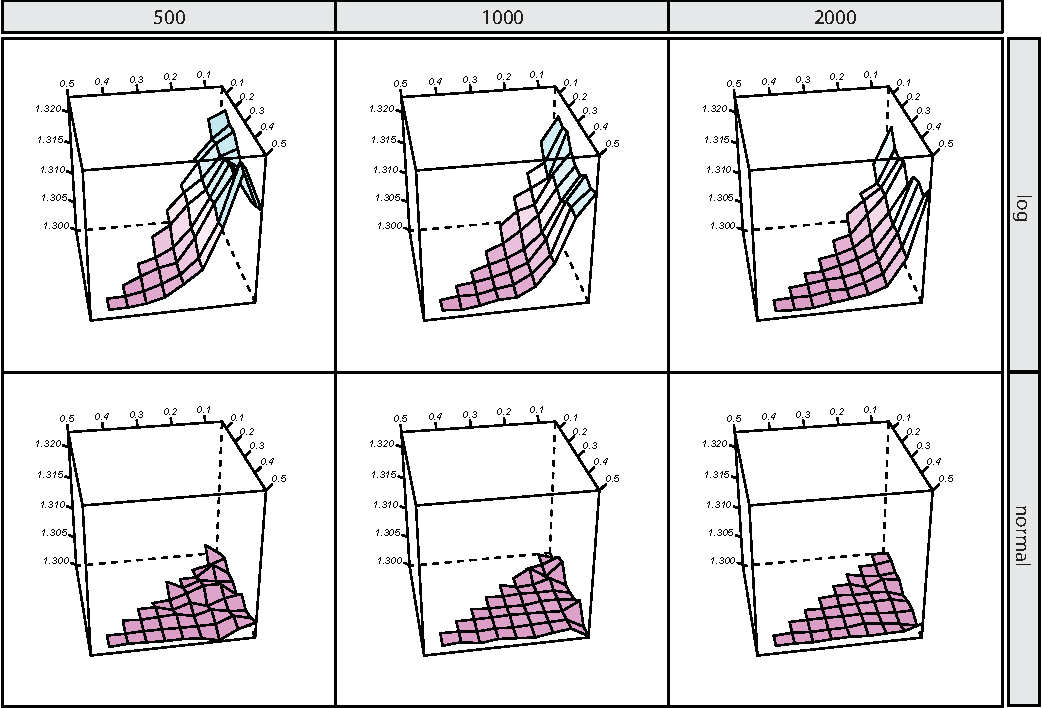
\includegraphics[width=5in]{Chapter3/fdr_5pc_wireframe.pdf}
\caption[Violation of assumptions of normality]{Results from Monte Carlo simulations showing the effect of allele frequency ($x$- and $y$-axes) on the inflation of test statistics ($z$-axis) when assumptions of normality are violated. The values of the wireframe plot are the $5^{th}$ percentile of the most extreme $-\log_{10}p$ values from $10^{5}$ pairwise tests with null models simulated at two loci with frequencies corresponding to the $x$- and $y$-axes. The top row of boxes shows the effect of using a log-normally distributed phenotype, and the bottom row when using a normally distributed phenotype. Columns of boxes represent different sample sizes.}
\label{fig:mc_af}
\end{center}
\end{figure}

\begin{figure}
\begin{center}
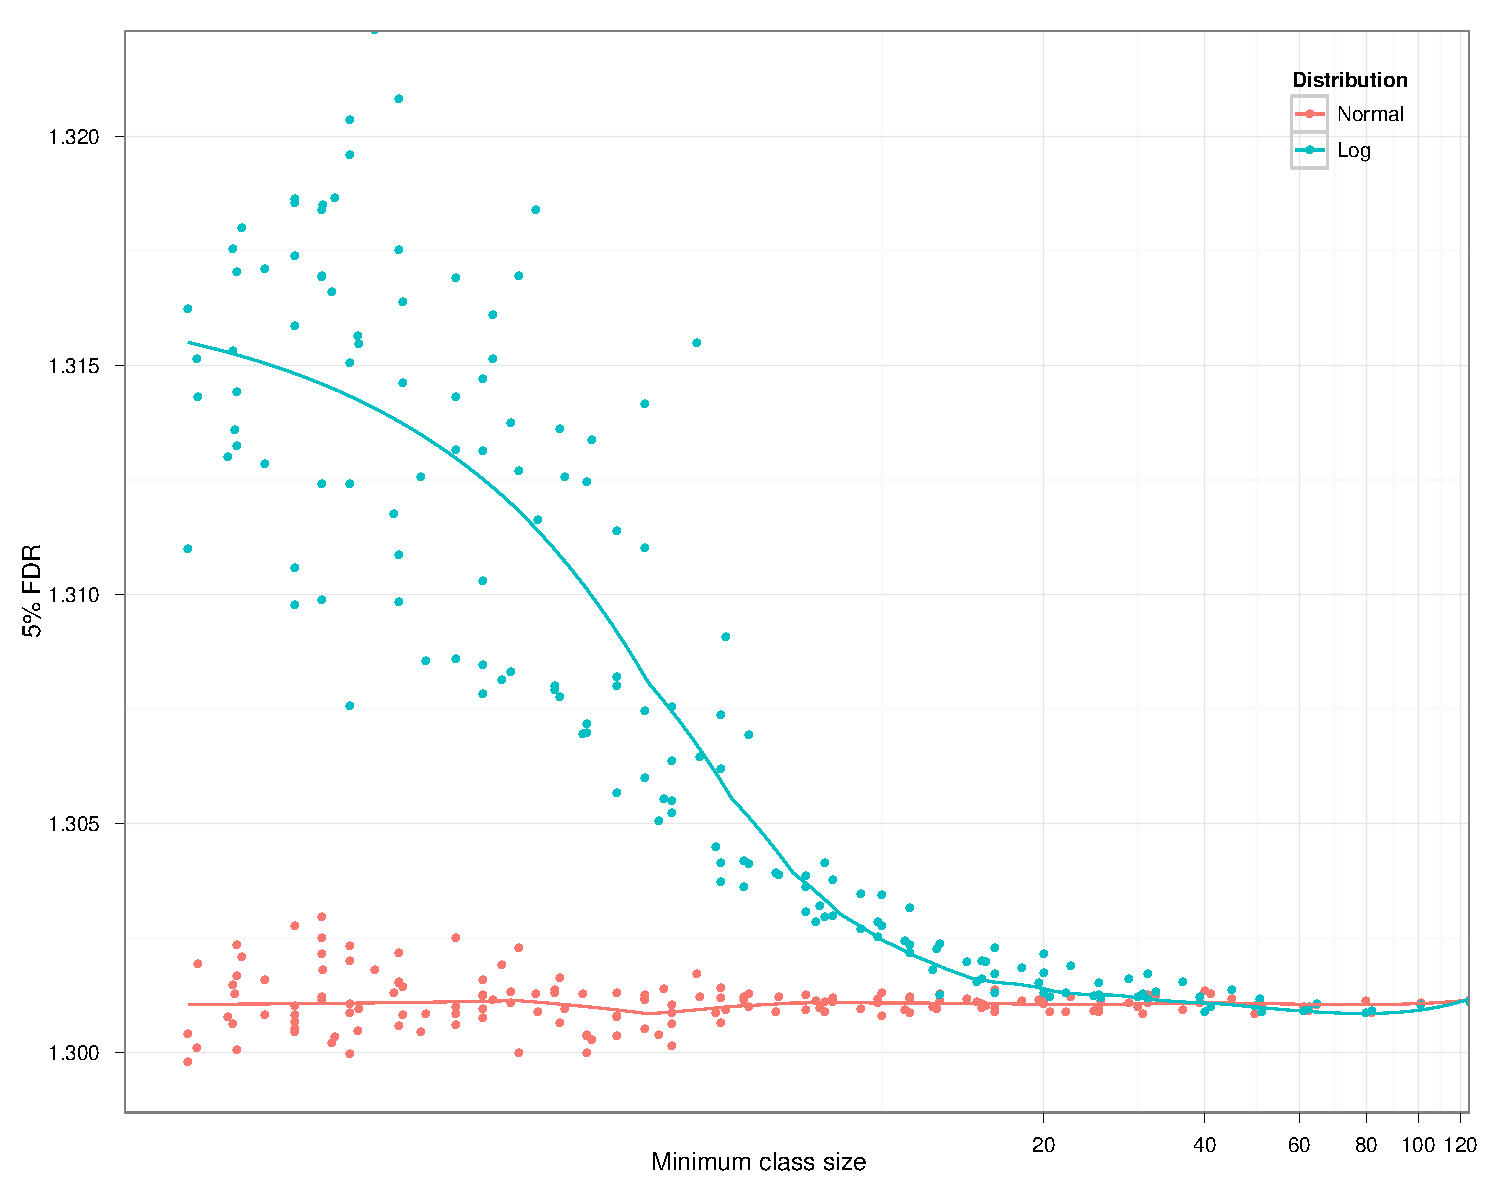
\includegraphics[width=5in]{Chapter3/inflation_vs_n.pdf}
\caption[Effect of minor class size on inflation]{The effect of the minimum non-zero genotype class size ($x$-axis, log scale) on the inflation of the test statistic for 8 d.f. epistatic tests. Data is taken from figure \ref{fig:mc_af}, demonstrating a clear trend between small class sizes and inflated test statistics for non-normal phenotypes.}
\label{fig:mc_classsize}
\end{center}
\end{figure}


The original dataset used for the permutation analysis (described in section \ref{bmi_data}) has been extensively analysed for genetic variation in BMI (Wei \emph{et al.} 2011, in preparation), and the results from these simulations may be important in their interpretation. Raw BMI values are generally skewed, resembling the log transformed distributions that were used as an example for the violation of normality in figure \ref{fig:mc_af}, and in general the most robust method to correct for non-normality is to use the method of rank transformation. Table \ref{tab:bmi_results} demonstrates the liability for false positives to occur when normality is violated in this manner. Most notably, many pairwise interactions were mined with $- \log_{10}p$-values sufficiently extreme to surpass the stringent Bonferroni correction of $11.95$. However, upon reanalysis following rank transformation of the phenotype these test statistics are significantly diminished. While few observations in certain genotype classes result in inflation, as in this case, it is important to note that under conditions of normality there is no such liability.

\begin{table}
  \begin{center}
  \rowcolors{3}{tableShade}{white}
  \begin{threeparttable}
  \caption{\label{tab:bmi_results}False positives from epistatic searches in BMI}
    \begin{tabular}{rrrrr}
    \toprule
SNP 1 & SNP 2 & MGC \tnote{a} & Raw $p$-value ($-\log_{10}$) \tnote{b} & Corrected $p$-value ($-\log_{10}$) \tnote{c} \\
\midrule
rs10789450 & rs1857985 & 6 & 13.82 & 9.87 \\
rs1217394 & rs826911 & 7 & 12.47 & 8.59 \\
rs9809255 & rs1857985 & 3 & 12.23 & 7.79 \\
rs10758713 & rs1857985 & 3 & 12.06 & 8.74 \\
rs1857985 & rs7342676 & 3 & 12.60 & 8.56 \\
rs1857985 & rs12927233 & 6 & 12.74 & 9.60 \\
rs755647 & rs2267271 & 4 & 12.61 & 8.08 \\
\bottomrule
\end{tabular}
\begin{tablenotes}{\footnotesize
\item[a] Minimum genotype class size (non-zero)
\item[b] Returned from scan using non-normalised phenotype
\item[c] Returned from scan using rank transformed phenotype}
\end{tablenotes}
\end{threeparttable}
\end{center}
\end{table}


\subsection{Permutation analyses}

Currently, there are very few exhaustive searches for epistasis being performed, and when they are being used they typically employ very conservative significance thresholds, such as the Bonferroni correction. Some efforts have been made to adjust this based on the estimated number of effective tests being performed \citep{Becker2011}, but in reality the behaviour of the extreme tail of the distribution when a very high number of multiple tests is being performed is unknown, nor is the true genomic correlation structure amongst these tests. Here, permutation analysis was used as the most direct way for answering these questions. 

The results from the permutation analysis are shown in figures \ref{fig:perm_density} and \ref{fig:thresh_error}, and table \ref{tab:perm_results}. There are several important conclusions that can be drawn from this analysis. Most importantly, the Bonferroni correction is shown to be overly conservative, and that using a scalar correction factor as in \citet{Becker2011} does not fully account for the asymptotic behaviour of the effective number of tests as SNP density increases (as shown in \citet{Dudbridge2008}).

\begin{figure}
\begin{center}
\includegraphics[width=5in]{Chapter3/thresh_error.pdf}
\caption[Empirical estimates of 2D search thresholds]{As depicted in figure \ref{fig:perm_density}, the 5\% family-wise FDR based threshold can be calculated from the distribution of maximum values from permutations (central dots). Through bootstrap analysis (10,000 resamples per permutation set) two-tailed 5\% confidence intervals were obtained for each threshold estimate.}
\label{fig:thresh_error}
\end{center}
\end{figure}

\begin{sidewaysfigure}
\begin{center}
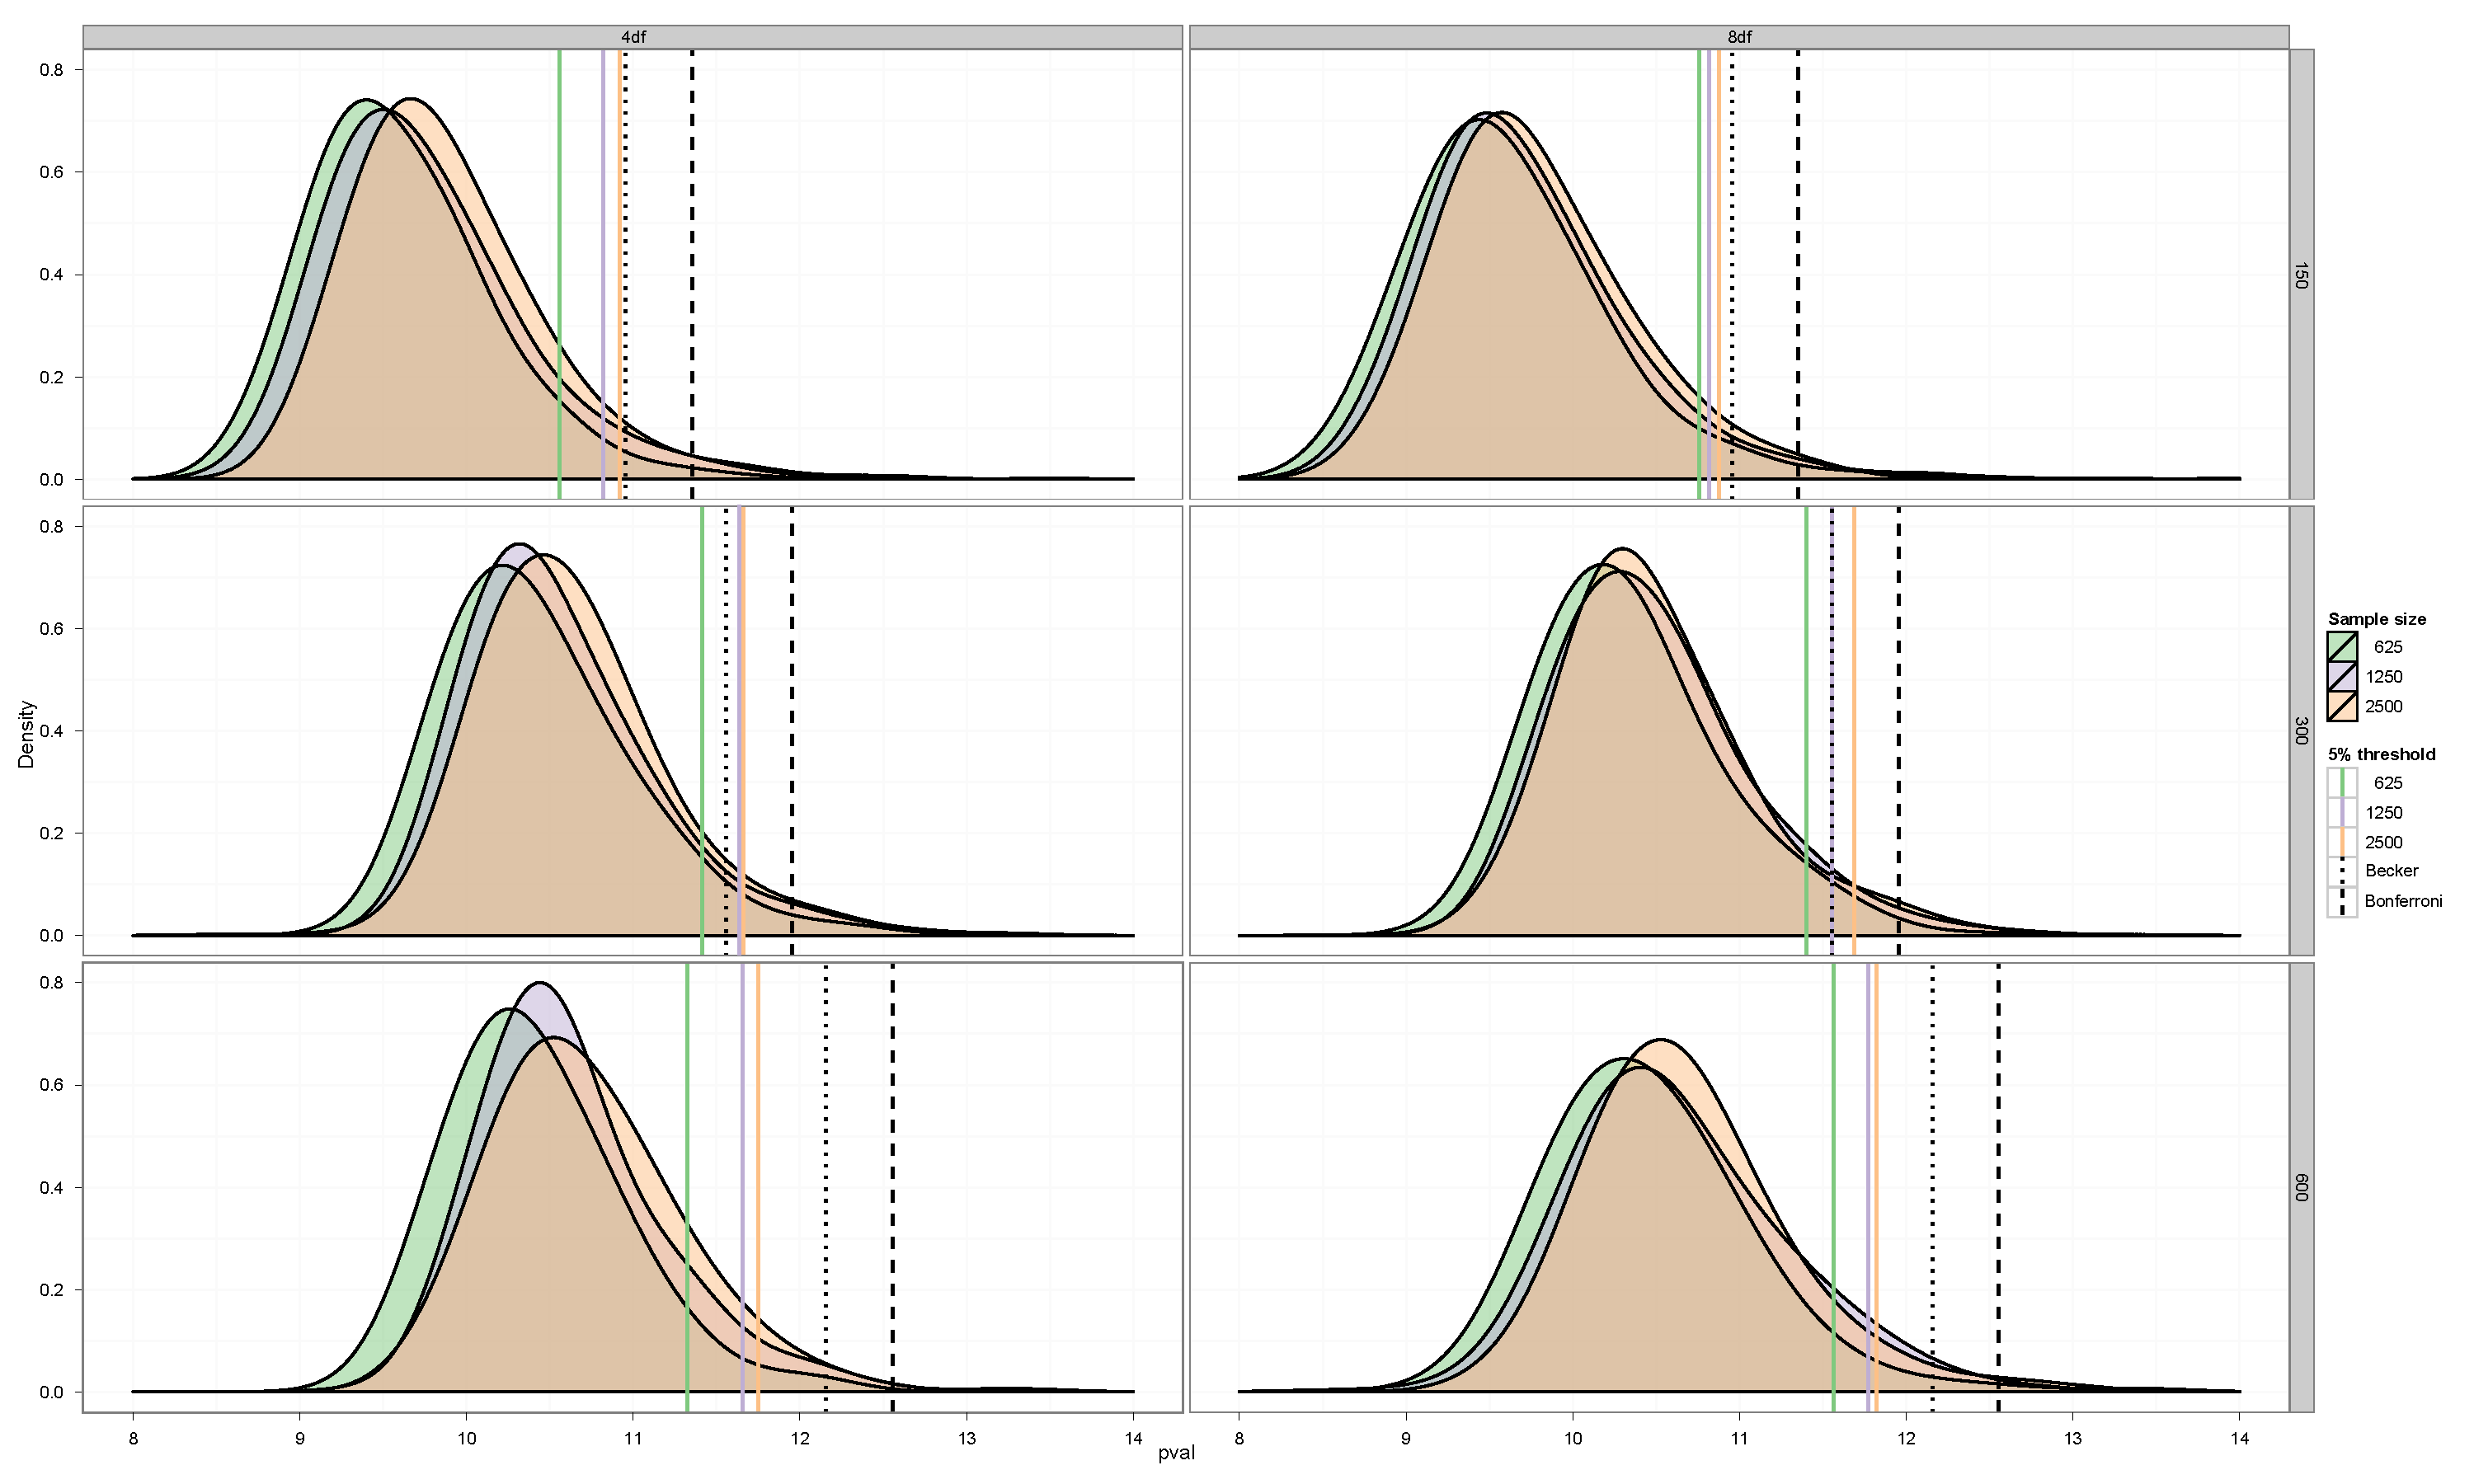
\includegraphics[width=8in]{Chapter3/perm_density.pdf}
\caption[Distribution of test statistics from permutation analysis]{Hundreds of permutations (table \ref{tab:perm_results}) were performed for two dimensional scans under varying testing conditions of SNP chip density (rows of boxes), sample size (distribution fill colour), and test parameterisation (columns of boxes). Each curve is a smoothed density of the top test statistics retrieved from each permutation representing its testing conditions. Vertical lines represent $5\%$ family-wise false discovery thresholds calculated for different sample sizes (colours), or for the extant methods of the Becker correction (dots) \citep{Becker2011} or Bonferroni correction (dashes).}
\label{fig:perm_density}
\end{center}
\end{sidewaysfigure}

\begin{sidewaystable}
  \begin{center}
%  \rowcolors{3}{tableShade}{white}
  \begin{threeparttable}
  \caption{\label{tab:perm_results}Summary of permutation results}
    \begin{tabular}{rrrrrrrrrrr}
    \toprule
Density & Sample size & Permutations & Tesla S1070 \tnote{a} & Tesla S2080 \tnote{a} & \multicolumn{4}{c}{5\% threshold} & \multicolumn{2}{c}{Effective SNPs \tnote{c}}  \\
& & & & & Bonferroni & Becker & 4 d.f. \tnote{b} & 8 d.f. \tnote{b} & 4 d.f. & 8 d.f. \\
\midrule
\multirow{3}{*}{150000} & 2476 & 1000 & 1:48 & 0:45 & \multirow{3}{*}{11.35} & \multirow{3}{*}{10.95} & 11.10 & 11.07 & 112762 & 109441 \\
& 1250 & 1000 & 0:56 & 0:22 & & & 11.05 & 11.10 & 105947 & 112472 \\
& 625 & 1000 & 0:28 & 0:11 & & & 10.97 & 10.90 & 96596 & 89496 \\
\midrule
 \multirow{3}{*}{283971} & 2476 & 1000 & 6:05 & 2:43 &  \multirow{3}{*}{11.95} &  \multirow{3}{*}{11.56} & 11.66 & 11.69 & 213480 & 221229 \\
& 1250 & 1000 & 3:08 & 1:20 & & & 11.65 & 11.55 & 212468 & 188973 \\
& 625 & 1000 & 1:35 & 0:39 & & & 11.41 & 11.40 & 160929 & 159168 \\
\midrule
 \multirow{3}{*}{600000} & 2476 & 500 & 29:42 & 11:57 & \multirow{3}{*}{12.56} & \multirow{3}{*}{12.16} & 11.77 & 11.79 & 243439 & 249695 \\
& 1250 & 500 & 15:10 & 6:04 & & & 11.67 & 11.77 & 216002 & 241078 \\
& 625 & 500 & 7:45 & 3:12 & & & 11.33 & 11.55 & 145732 & 189233 \\
\bottomrule
\end{tabular}
\begin{tablenotes}{\footnotesize
\item[a] Timings shown as \emph{hours}:\emph{minutes} per permutation as performed by {\tt epiGPU} using different hardware.
\item[b] Empirical thresholds for 5\% family-wise false discovery rates calculated from permutation results.
\item[c] Effective number of SNPs being tested based on empirical thresholds from permutation analysis.
}\end{tablenotes}
\end{threeparttable}
\end{center}
\end{sidewaystable}

Secondly, there is no significant inflation of low frequency SNPs among the permuted searches. Figure \ref{fig:mafdens} shows that the distribution of allele frequencies comprising the top 100 SNP pair hits from each permuted scan is similar to the distribution of all SNPs in the SNP panels. This is an important result, because it allows researchers to have equal confidence in hits comprising SNPs with rare frequencies as with those with intermediate frequencies, at least from the perspective of there being no artificial statistical inflation.

\begin{figure}
\begin{center}
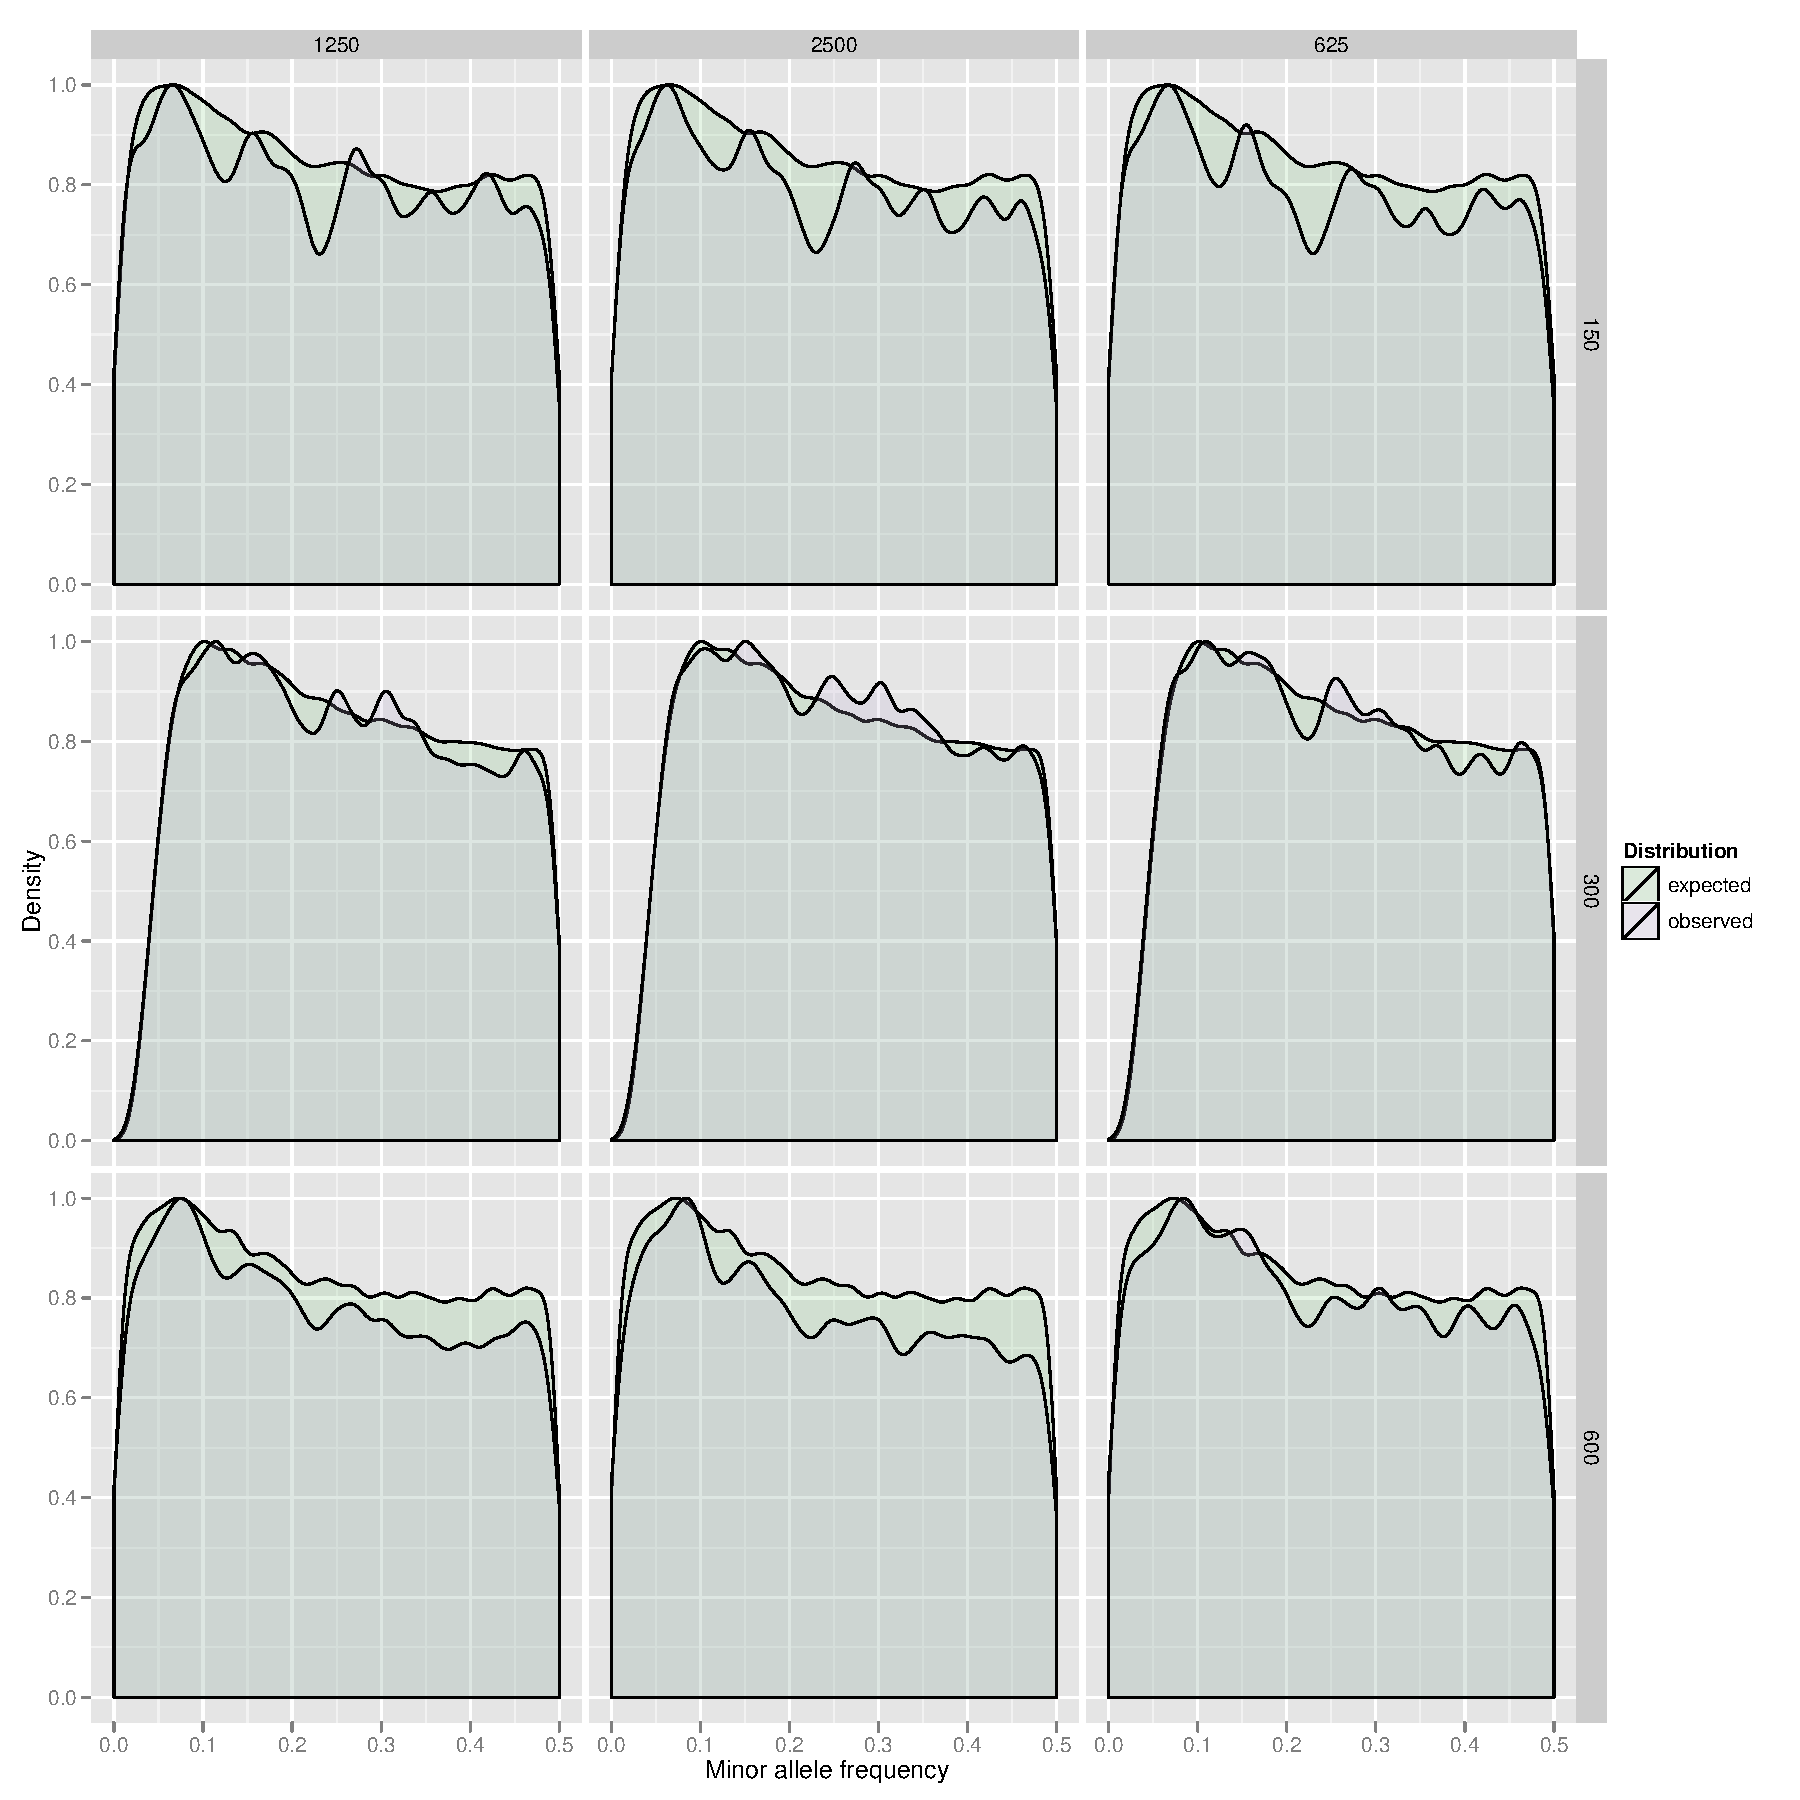
\includegraphics[width=5in]{Chapter3/mafdens.pdf}
\caption[Observed vs expected SNP frequency densities]{The frequency density of the SNP chip (red) is plotted along with the density of frequencies of the 100 most significant SNPs obtained from each permutation for 8 d.f. tests. Columns of boxes represent sample size, and rows represent SNP density ($\times 1000$).}
\label{fig:mafdens}
\end{center}
\end{figure}

Thirdly, in most cases there is no discernible impact of the test parameterisations on the thresholds. When the sample size is smallest there is a slight decrease in the estimated threshold for 4 d.f. tests. This is expected because the actual number of tests performed is expected to drop because SNP pairs that do not have observations for all 9 genotype classes are omitted from the scan for 4 d.f. tests, but not for 8 d.f. tests.

Finally, increasing sample size has an increasing effect on the threshold. While the data is insufficient to make a strong statement about this, there is a tendency for the elevation of the threshold from 625 to 1250 observations to be larger than from 1250 to 2476, and this may indicate an asymptotic relationship (figure \ref{fig:thresh_error}). To speculate on the reason for this relationship is difficult, but the following observations can be made regarding the three variables involved in the test statistic: the actual sample size $n$, the average variance explained by all tests in the scan $SS_{W} / (SS_{W}+SS_{B})$, and the average number of parameters per test $g$ (this will vary when small sample sizes have more missing genotype classes). In a background of two factors remaining fixed, the \emph{approximate} behaviours of the third factors can be described as:

\begin{eqnarray}
-\log \left ( f \left (
\frac{
 SS_{W}  (g - 1)^{-1}
}
{  SS_{B} (n - g)^{-1}
}; g - 1, n - g
\right ) \right )
& \propto &
 n \\
& \propto &
SS_{W} / (SS_{W} + SS_{B}) \\
& \propto &
-\log(g)
\label{eq:ftest_n}
\end{eqnarray}
where $f(x; d_{1}, d_{2})$ is the probability density function for some random $F$-distributed variable $x$ with numerator and denominator degrees of freedom $d_{1}$ and $d_{2}$ respectively. First of all smaller values of $n$ require more extreme data in order to achieve the same level of significance as those from larger sample sizes, however the actual distribution of $SS_{W} / (SS_{W} + SS_{B})$ from an exhaustive scan with respect to sample size is unknown, although one could intuitively suggest an inverse correlation. Secondly, the relationship between sample size and the number of parameters will follow an asymptotic function 
\begin{equation}
\lim_{n \to \infty} \bar{g} = 9
\end{equation}
so as sample size increases, the increase in $\bar{g}$ will oppose the propensity to achieve extreme $p$-values due to increased sample size. The relationship is complex and without knowing the underlying distribution for each variable it is difficult to deterministically support the empirical observation of the effect of sample size on the threshold. For the purposes of the following analysis it is assumed that it is indeed a product of some asymptotic function, although further analysis will be required to confirm this.

Although the relaxation of significance thresholds when calculated from permutation is fairly modest in these examples, the conclusion may have a further reaching utility. For each of the 18 permutation sets (3 sample sizes $\times$ 3 SNP densities $\times$ 2 test parameterisations; table \ref{tab:perm_results}) bootstrap analysis was performed to ascertain confidence intervals for the 5\% family-wise FDR (figure \ref{fig:thresh_error}). Naturally, the number of permutations performed here are constrained by computational resources, and so the results provide an approximation to the effective number of tests that will become more robust with more permutations. Nevertheless, it may be useful to attempt to derive an empirical relationship between the threshold, SNP density, and sample size. Assuming that the effect on the threshold from SNP density and sample size are independent of one another, and that they each follow an exponential asymptotic relationship toward some theoretical maximum number of tests given infinite SNP density, non-linear least squares (NLS) were performed to ascertain the parameters to the model, using the data from the $10000$ bootstrap samples for each of the 18 permutation sets.

The limit to the asymptote (the maximum number of tests with infinite SNP density and sample size) was estimated theoretically (rather than as a parameter in the NLS calculation). From the result in \citet{Dudbridge2008} the effective number of independent regions in a one dimensional GWAS is estimated to be $693138$, therefore the effective number of independent tests in a two dimensional GWAS at infinite SNP density is $\frac{693138 \times 693137} {2} = 2.4 \times 10^{11}$, giving a theoretical maximum $-\log_{10} p$-value of $12.68$. From this, for $n$ sample size and $M$ SNPs in the array the family-wise threshold $p_{T}$ was modelled as 

\begin{equation}
-\log_{10}(p_{T}) = a - a \left ( 
 s_{1} \exp \left ( 
  \frac {\ln(n) } { s_{2} } \right )
 + s_{3} \exp \left (
  \frac{ \ln(M)} {s_{4}} \right ) 
\right )^{-1}
\label{eqn:general_threshold}
\end{equation}
where the asymptotic limit was set to $a = 12.68$, and the following parameter estimates from NLS were obtained:
\begin{eqnarray}
s_{1} & = & 0.0258 \nonumber \\
s_{2} & = & 1.72 \nonumber \\
s_{3} & = & 0.0379 \nonumber \\
s_{4} & = & 2.33. \nonumber
\end{eqnarray}
This relationship is depicted in figure \ref{fig:threshold_function}.

\begin{figure}
\begin{center}
\includegraphics[width=5in]{Chapter3/threshold_function.pdf}
\caption[Estimation of 2D thresholds in the general case]{The wireframe maps the empirically derived relationship obtained in equation \ref{eqn:general_threshold}. The $z$-axis represents the estimated threshold for some given combination of sample size ($x$-axis) and SNP density ($y$-axis), and tending towards an asymptotic limit of $12.68$.}
\label{fig:threshold_function}
\end{center}
\end{figure}

% why is becker wrong?

\section{Discussion}

The question of where to set significance thresholds for whole genome searches is a long standing problem, and while the solutions are still perhaps incomplete in the one dimensional case, very little attention has been directed specifically to the context of epistasis. This chapter assesses the impact of non-normality on the inflation of type 1 errors in epistatic scans, presents the results from permutation analyses on exhaustive two dimensional searches, and attempts to derive significance thresholds that accurately reflect the effective number of tests being performed.

The first main conclusion is that it is imperative that a normal phenotype is used in order to be confident of avoiding type 1 error inflation. Specifically, the simulations here were concerned with the impact of outliers on the distribution of test statistics mainly because this was representative in the case of searches for epistatic variants contributing to the BMI variance in populations (Wei \emph{et al.} 2011, in preparation). It was shown that SNP pairs with low genotype counts were susceptible to type 1 error inflation, but such was not the case when the distribution of the phenotype was normalised using rank transformation.

In terms of the permutation analysis, the broad conclusion that can be based on these results is that the correlation structure between SNPs, as well as between pairwise tests, is relatively high, with the most extreme case showing a reduction in the threshold from the Bonferroni by almost an order of magnitude. However, although the Bonferroni approach is most conservative, the magnitude of multiple testing as estimated through permutation is still extremely high. It is perhaps not until the SNP array becomes very dense (\emph{e.g.} $>300000$ SNPs), and permutation thresholds become constrained by the asymptote (figure \ref{fig:threshold_function} and equation \ref{eqn:general_threshold}), that the use of permutation thresholds will constitute a significant advantage in power as the Bonferroni thresholds will continue to grow quadratically. Indeed, at lower SNP densities the approximate thresholds derived by \citet{Becker2011} that simply scale the number of multiple tests linearly (by 0.44) are reasonably accurate. Incidentally, the permutation results that most closely matched the Becker threshold came from the 300000 SNP density, however the Becker threshold was based on a 500000 SNP array. It could be argued that the method of performing Monte Carlo draws on relatively small sections of the genome resulted in an underestimate of the long range correlation structures, where although each long range SNP pair will be lowly correlated, there is an extremely large volume of these pairs in total.

Performing the permutations, even with the availability of GPU compute clusters, was extremely computationally demanding, and most researchers will not have access to this type of hardware. Furthermore, even with such hardware, as the SNP density increases the computational time required becomes unmanageable, and ostensibly at the higher densities the permutation based thresholds are of most utility. By using the general function (equation \ref{eqn:general_threshold}) to estimate significance thresholds for larger sized studies, it should be possible to impose a meaningful statistical threshold that takes into consideration the effective number of tests being performed in the scan as well as the impact of sample size. However there are some potential issues with using an empirically derived function. First, there are significant differences in LD structure between species, SNP manufacturers (\emph{e.g.} Affymetrix and Illumina \citep{Gao2010, Becker2011}, tagging or non-tagging SNPs \citep{Stram2004, Halperin2005}), and human ethnicities \citep{TheInternationalHapmapConsortium2005}. Second, imputation was used for the acquisition of the 600000 SNP array, and one potential issue that might arise from this is that the imputation algorithm may not capture local recombination events or population specific polymorphisms, and therefore cause an overestimation of the between-SNP correlation structure. Although the estimate of the asymptotic limit is unlikely to increase, the overestimation of correlation will result in a gentler growth toward the limit, and systematically underestimate thresholds for all densities above $\sim$ 300000 SNPs. While the latter problem can be resolved simply by using more data points and using only directly genotyped data rather than imputed data, the former problem is less easily amenable. Perhaps the most direct method would be through extensive permutation analyses under the varying conditions. Finally, the threshold estimates from the permutations are unlikely to be particularly accurate because they are based on only 1000 (or 500) randomisations. Desirable would have been to increase these numbers by an order of magnitude, and then perhaps the assumed asymptotic relationships within sample size (should they be real) and SNP densities would become more robust.

A third potential issue is that the estimate of the asymptotic limit $a=12.68$ may be overly stringent, because as alluded to in \citet{Becker2011} the effective number of tests being performed in a two dimensional scan depends on two principles - the number of independent regions, and the correlation between tests that involve one SNP, $i$, against $M$ other SNPs. The estimate of $a$ accounts for the first principle, but it does not consider the second. Intuitively this may be quite significant, because for example the marginal effect of SNP $i$ will be tested $M$ times. Although the correction factor for this was estimated to be fairly close to $1$ (\emph{i.e.} relatively insignificant correlations), a more formal investigation into this could be made. For example, a Monte Carlo based simulation that compared the Bonferroni threshold against a permutation based threshold using a panel of completely uncorrelated SNPs should find no difference if this latter type of correlation is low.

From a different perspective, one concern with high dimensional testing is that of exhausting the possible combinations of genotype-phenotype maps. For example, in the example of canalisation, where there are ostensibly two groups of individuals - those homozygous mutant at both loci (\emph{e.g.} high phenotype), and those who are not (low phenotype) - in a sample size of $n = 100$ where $r = 10$ are the double homozygotes the possible number of combinations is $C_{(100,10)} = 1.73 \times 10^{13}$, where
\begin{equation}
C_{(n,r)} = \frac{n!}{r!(n-r)!}.
\end{equation}
so given sufficient effective number of tests, the most extreme assortment of phenotypes into high and low groups will inevitably occur, such that no true biological interaction of the same map could possibly be more statistically extreme. Counteracting this is straightforward, as sample size increases the number of combinations expands rapidly, for example $C_{(1000,10)}  = 2.63 \times 10^{23}$, but this may remain a problem for very high dimensional searches (\emph{e.g.} with four way interactions, $500000^4 = 6.25 \times 10^{22}$), and several approaches that do attempt to explore higher order interactions, albeit not exhaustively, may be liable to such an issue. Relatedly, to partition the phenotypes according in the most extreme manner, such that the highest values are in one group and the lowest in another group, there is only one unordered arrangement where this could occur. But the number of arrangements with only a certain proportion of the more extreme phenotypes being assorted, rather than the exact set of the most extreme, into a single group will be large, so the combinatorial eventuality of `good' evidence for interaction may still be present. If such a process were at work, it would be most visible in the situation with the densest SNPs and the smallest sample size where one would expect to see many extreme results elevating the threshold, however there is clear evidence that the permutation threshold is actually reduced when sample size is reduced, suggesting that the search is not becoming saturated in combinatoric terms. The estimation of threshold values based on sample size has been discussed previously \citep{TheWellcomeTrustCaseControlConsortium2007}, where the logic has been that as sample size decreases then power decreases, so evidence for association should be more conservative. The results from these permutations suggest otherwise, that as sample size decreases the most extreme $p$-values that occur by chance are smaller. Further work is required to ascertain the underlying cause for this.

Anecdotally, the most extreme result from all permutations gave a $p$-value of $3.9 \times 10^{-16}$, and many were an order of magnitude more extreme than even the Bonferroni correction. It should be noted that family-wise thresholds only promise that from a set of multiple comparisons the chance of finding exactly one more extreme result is some value of $\alpha$, and they do not inform the distribution of $p$-values that comprise the $\alpha$ false discoveries. Therefore, in this context further calculation is required in order to believe a particularly extreme result with any greater level of confidence than the nominal $\alpha$ value. 

To summarise, the computations performed here demonstrate that Bonferroni corrections are overly conservative, and the \citet{Becker2011} approximation is only valid at low SNP density. Yet, the presumably more accurate empirical distributions of test statistics from exhaustive pairwise scans are still very stringent. Although their use will improve power to some extent over existing practices, particularly with sequence data, the most effective direction is to increase sample sizes, and to focus on improving the power of the statistical methodology.
